\chapter{monai\_valley}

\section{Purpose}

Redo the monai valley experiment from Costas E Synolakis (p45, 3.4)\cite{Costas2007}.

\section{Description}

\subsection{Mesh and geometry}

Size of the model: rectangle (3.4m x 5.5m)

Nodes   12989
Elements  25553

The Figure~\ref{fig:monai:mesh} shows the mesh of the study.
\begin{figure}
\centering
\includegraphicsmaybe{[width=.6\textwidth]}{../img/Mesh.png}
\caption{Mesh of the study}\label{fig:monai:mesh}
\end{figure}

The Figure~\ref{fig:monai:bathy} shows the bathymetrie of the study.
\begin{figure}
\centering
\includegraphicsmaybe{[width=.6\textwidth]}{../img/Bathy.png}
\caption{Bathymetrie of the study}\label{fig:monai:bathy}
\end{figure}

\subsection{Boundary}

The Figure~\ref{fig:monai:boundaries} shows the boundaries of the study and the incident wave.
\begin{figure}
\centering
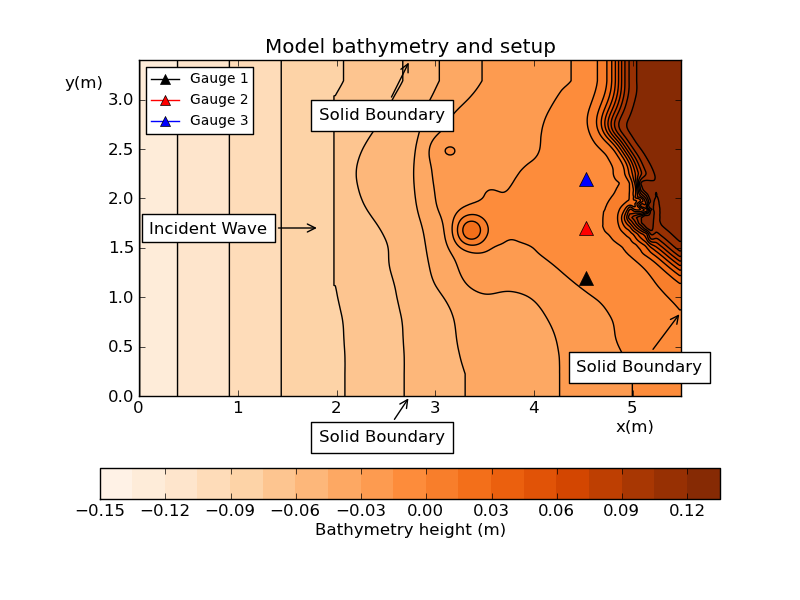
\includegraphics[width=.6\textwidth]{img/boundaries.png}
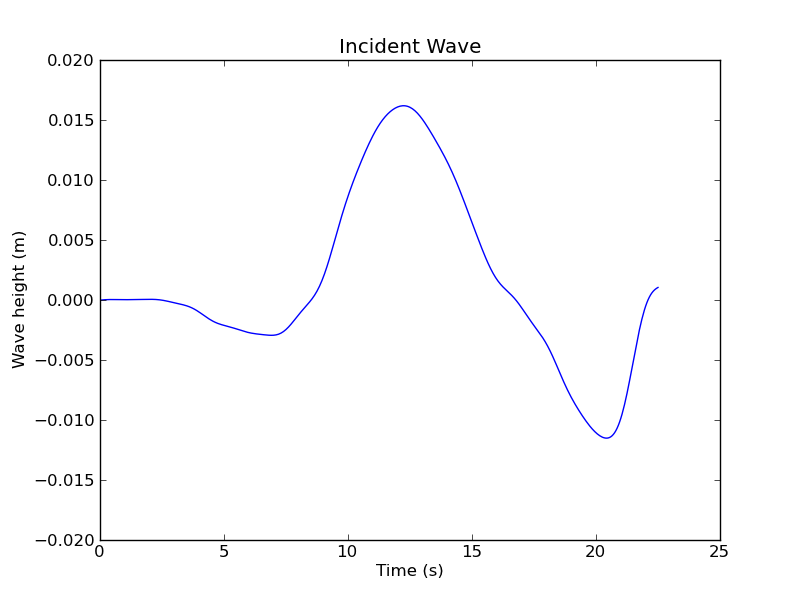
\includegraphics[width=.6\textwidth]{img/wave.png}
\caption{Boundaries of the study}\label{fig:monai:boundaries}
\end{figure}

Bottom: Chezy's Law

Friction coefficient: 180

\section{Physical parameters}

Turbulence: Constant viscosity equal to zero

\section{Numerical parameters}
1.7 Algorithm
\begin{itemize}
\item Type of element: P1 triangle for h and for velocity
\item Solver:  GMRES
\item Accuracy:  $10^{-6}$
\item Finite volume scheme:  Kinetic order 2
\item Equations: Saint-Venant VF
\end{itemize}

Time data:
\begin{itemize}
\item Time step: 0.0005
\item Simulation duration: 22.5
\end{itemize}

\section{Results}

%fig vel
The Figure~\ref{fig:monai:vel} shows the velocity vectors.
\begin{figure}
\centering
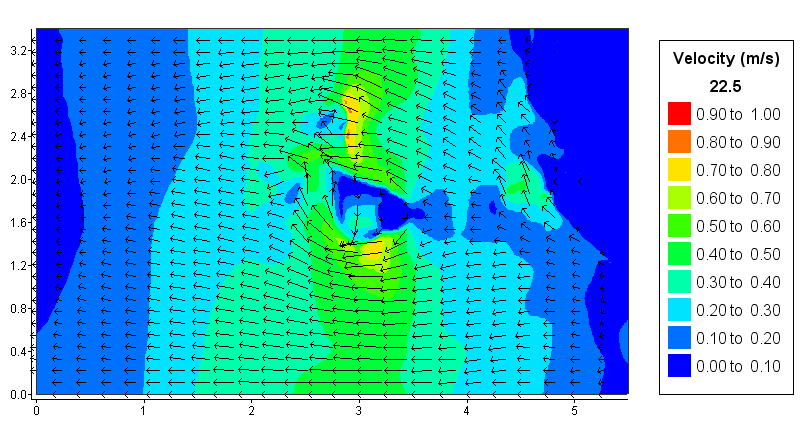
\includegraphics[width=.6\textwidth]{img/vel.png}
\caption{Velocity vectors over the free surface}\label{fig:monai:vel}
\end{figure}

We compare the model and experiment free surface at gauges 1,2 and 3

The Figure~\ref{fig:monai:res} shows the comparison with the benchmark data.
\begin{figure}
\centering
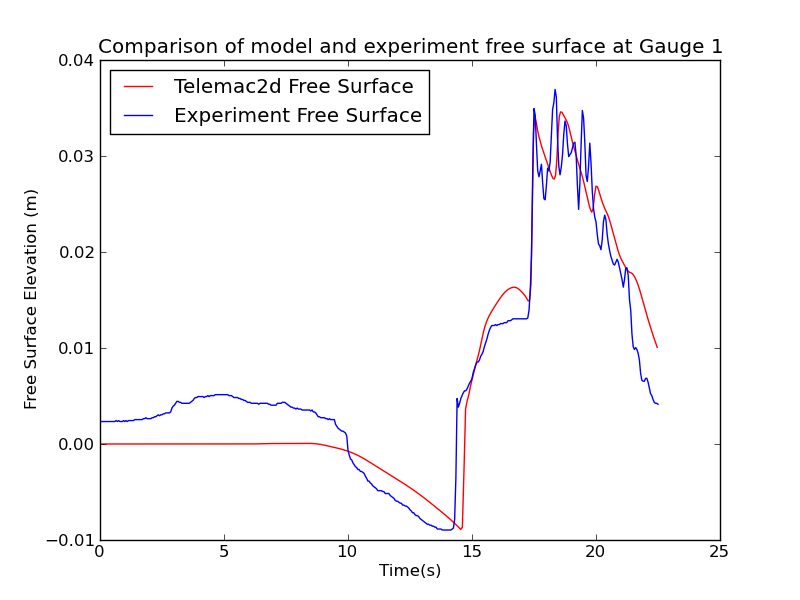
\includegraphics[width=.8\textwidth]{img/res_g1.png}
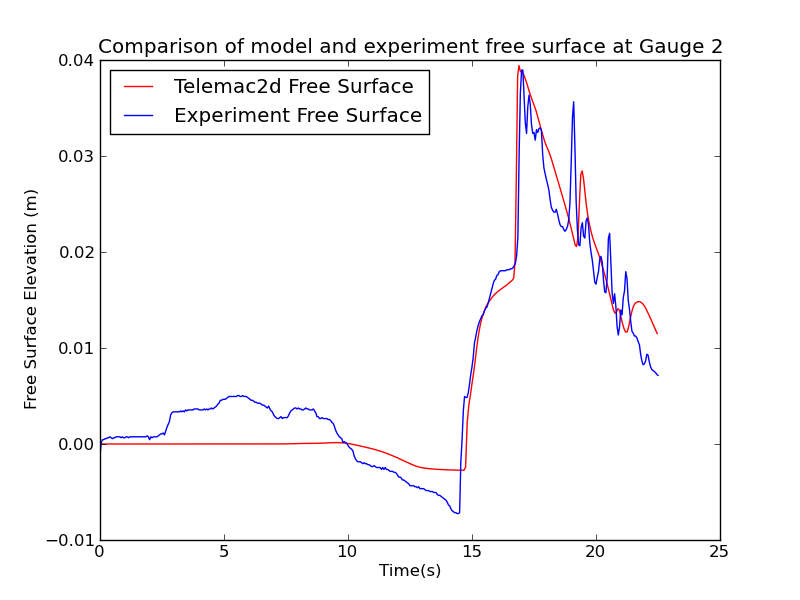
\includegraphics[width=.8\textwidth]{img/res_g2.png}
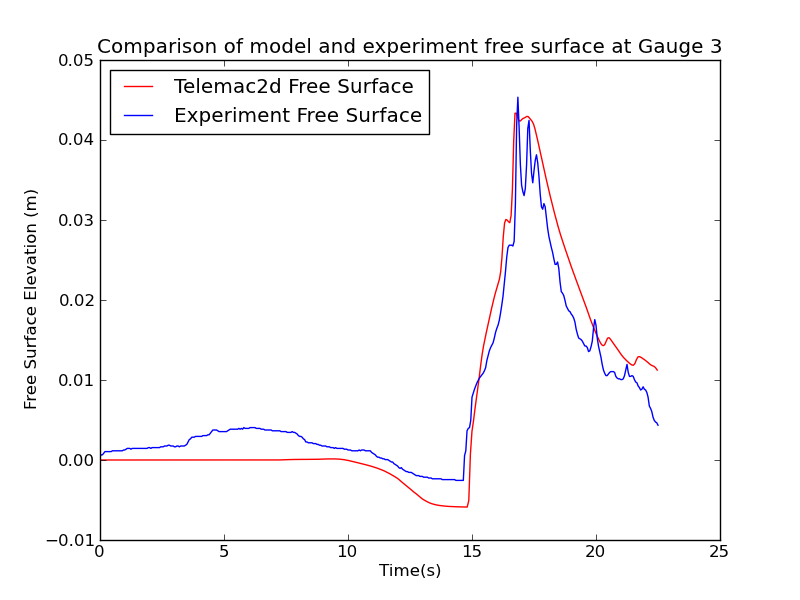
\includegraphics[width=.8\textwidth]{img/res_g3.png}
\caption{Comparaison of the results}\label{fig:monai:res}
\end{figure}
